\documentclass[aps,twocolumn,secnumarabic,balancelastpage,amsmath,amssymb,nofootinbib]{revtex4}
% \documentclass[aps,twocolumn,secnumarabic,balancelastpage,amsmath,amssymb,nofootinbib]{revtex4}

% Documentclass Options

% nobalancelastpage doesn't attempt to equalize the lengths of the two columns
% on the last page as might be desired in a journal where articles follow one
% another closely
% amsmath and amssymb are necessary for the subequations environment among
% others secnumarabic identifies sections by number to aid electronic review
% and commentary. nofootinbib forces footnotes to occur on the page where they
% are first referenced and not in the bibliography

% \usepackage{lgrind}        % convert program listings to a form includable in a LaTeX document
\usepackage{chapterbib}    % allows a bibliography for each chapter (each labguide has it's own)
\usepackage{color}         % produces boxes or entire pages with colored backgrounds
\usepackage{graphics}      % standard graphics specifications
\usepackage[pdftex]{graphicx}      % alternative graphics specifications
\usepackage{longtable}     % helps with long table options
\usepackage{epsf}          % old package handles encapsulated post script issues
\usepackage{bm}            % special 'bold-math' package
\usepackage{tikz}
\usepackage{asymptote}     % For typesetting of mathematical illustrations
\usepackage{subfigure}

% \usepackage{thumbpdf}

\usepackage[colorlinks=true]{hyperref}  % this package should be added after all others
% use as follows: \url{http://web.mit.edu/8.13}
\newcommand{\drelectron}[1]{\node at #1 [circle, draw, inner sep=0pt, minimum size=1pt] {\_}}
\newcommand{\ud}{\mathrm{d}}
\newcommand{\ue}{\mathrm{e}}
\newcommand{\ui}{\mathrm{i}}
\newcommand{\res}{\mathrm{Res}}
\newcommand{\Tr}{\mathrm{Tr}}
\newcommand{\dsum}{\displaystyle\sum}
\newcommand{\dprod}{\displaystyle\prod}
\newcommand{\dlim}{\displaystyle\lim}
\newcommand{\dint}{\displaystyle\int}
\newcommand{\fsno}[1]{{\!\not\!{#1}}}
\newcommand{\eqar}[1]
{
  \begin{align*}
    #1
  \end{align*}
}
\newcommand{\texp}[2]{\ensuremath{{#1}\times10^{#2}}}
\newcommand{\dexp}[2]{\ensuremath{{#1}\cdot10^{#2}}}
\newcommand{\eval}[2]{{\left.{#1}\right|_{#2}}}
\newcommand{\paren}[1]{{\left({#1}\right)}}
\newcommand{\lparen}[1]{{\left({#1}\right.}}
\newcommand{\rparen}[1]{{\left.{#1}\right)}}
\newcommand{\abs}[1]{{\left|{#1}\right|}}
\newcommand{\sqr}[1]{{\left[{#1}\right]}}
\newcommand{\crly}[1]{{\left\{{#1}\right\}}}
\newcommand{\angl}[1]{{\left\langle{#1}\right\rangle}}
\newcommand{\tpdiff}[4][{}]{{\paren{\frac{\partial^{#1} {#2}}{\partial {#3}{}^{#1}}}_{#4}}}
\newcommand{\tpsdiff}[4][{}]{{\paren{\frac{\partial^{#1}}{\partial {#3}{}^{#1}}{#2}}_{#4}}}
\newcommand{\pdiff}[3][{}]{{\frac{\partial^{#1} {#2}}{\partial {#3}{}^{#1}}}}
\newcommand{\diff}[3][{}]{{\frac{\ud^{#1} {#2}}{\ud {#3}{}^{#1}}}}
\newcommand{\psdiff}[3][{}]{{\frac{\partial^{#1}}{\partial {#3}{}^{#1}} {#2}}}
\newcommand{\sdiff}[3][{}]{{\frac{\ud^{#1}}{\ud {#3}{}^{#1}} {#2}}}
\newcommand{\tpddiff}[4][{}]{{\left(\dfrac{\partial^{#1} {#2}}{\partial {#3}{}^{#1}}\right)_{#4}}}
\newcommand{\tpsddiff}[4][{}]{{\paren{\dfrac{\partial^{#1}}{\partial {#3}{}^{#1}}{#2}}_{#4}}}
\newcommand{\pddiff}[3][{}]{{\dfrac{\partial^{#1} {#2}}{\partial {#3}{}^{#1}}}}
\newcommand{\ddiff}[3][{}]{{\dfrac{\ud^{#1} {#2}}{\ud {#3}{}^{#1}}}}
\newcommand{\psddiff}[3][{}]{{\frac{\partial^{#1}}{\partial{}^{#1} {#3}} {#2}}}
\newcommand{\sddiff}[3][{}]{{\frac{\ud^{#1}}{\ud {#3}{}^{#1}} {#2}}}

\begin{document}
\tikzstyle{every picture}+=[remember picture]
\title{Non-linear effect and patterns in the scattered beam of close resonance laser in a Rubidium vapor cell}
\author{Yichao Yu}
\email{yuyichao@mit.edu}
\homepage{http://yyc-arch.org/}
\date{\today}
\affiliation{MIT Department of Physics}

\begin{abstract}
  Nonlinear optics is an important branch of optics which studies the behavior of light in a nonlinear media in which the polarization is not a linear function of the electric field. The nonlinear effect in the media can cause interaction between light and an external field or even between two light beams for higher order nonlinear effects. These interactions give rise to the optical information processing that can possibly make computing faster using less energy. However, for classical nonlinear media, there is a compromise between non-linearity and reaction speed. Recently, people have been hoping on using quantum effect to design a fast and efficient non-linear media. Several ways have been proposed including using optical crystal and atomic energy levels. In our experiment, we studied the non-linear effect and pattern formation in a Rubidium vapor cell and partially reproduced one possible way of making an all-optics switch.
\end{abstract}

\maketitle
%%%%%%%%%%%%%%%%%%%%%%%%%%%%%%%%%%%%%%%%%%%%%%%%%%%%%%%%%%%%%%%%%%
\section*{Introduction}
Optical information processing, which uses light instead of electricity (like a modern computer), is thought to be one of candidates of next generation computing. It can be faster and also more energy efficient. The realization of such processing requires nonlinear media where the relation between polarization and electric field is no longer linear. In such media, the effective index of refraction as well as other properties can be affected by an external field or even another light beam which can be used to make electric-optics switches and even all-optics switches. These effects have been studied thoroughly in around 1980s and a lot of possible applications had been proposed. However, when using classical nonlinear media, there is a compromise between the reaction time and nonlinear coefficients. Materials like liquid crystal have really big nonlinear effect but they also have a reaction time in the order of $1$ms. Other media usually have a really small nonlinear effect and will require high light power to work. These properties are really limiting the advantage of optical information processing and making it impossible to use classical nonlinear media.

Recently, people have been trying to solve the problem using quantum physics and the control of energy levels. One possible way is using a optical crystal in which one can introduce and control the nonlinear effects by designing certain band structures. Another way is using a close resonance beam of certain atomic line. Using the strong interaction between light and atom close to resonance, a pattern forming effect had been observed in both experiment\cite{rb_exp} and simulation\cite{rb_sim} and the possible application of making all-optics switch has also been studied experimentally\cite{rb_switch}.

In our experiment, we have used a similar setup with that used in the all-optics switch\cite{rb_switch} and studied the light generated when two counterpropagating beams are close to resonance with the Rubidium atom in the cell. We were able to see several patterns appears in the generated light and partially reproduce some effect for the all-optics switch.

\section{Theory}
\subsection{Saturated absorption and non-linear effect.}
When a close resonance laser beam is interacting with atoms, part of the beam will be absorbed and scattered by the atoms. At the same time, if the intensity of the laser is strong enough, the stimulated emission will be comparable or stronger than the spontaneous emission, atoms will be pumped to the excited state, there will be almost equal number of atoms in the excited and ground states and the scattering will also reach a maximum. This effect is called saturated absorption and the intensity is called saturation intensity ($I_{set}$). Since the stimulated emission is important in this regime, the reaction to light of the atoms is not linear anymore and there can be interaction between multiple beams. Since the scattering is already saturated, the close resonance light will no longer be strongly absorbed which makes it possible to do observations.

\subsection{Scattering in a standing wave and interference rings.}
By using a mirror to retro-reflect the laser beam, we can create a standing wave in the cell. The distance between each wave crest where the constructive interference happens is half the incident wave length. Therefore, the phase of the light at each wave crest is alternating between $0$ and $\pi$ and the light scattered at each point will have the same phase relation. If the incident beam is red detuned the distance between wave crests will be larger than the wavelength of the wavelength scattered by the atoms and a interference ring can appear when the constructive interference condition is satisfied, i.e.,
\eqar{
  \lambda\cos\theta=&\lambda_0
}
where $\lambda$ and $\lambda_0$ are the wavelength of the incident beam and the atomic line respectively and $\theta$ is the angle between the incident beam and the ring. In the small detuning limit (also in the small angle limit because rings with a larger angle will get out of the region of the beam and therefore absorbed by the non-pumped atoms), this can be rewrite as,
\eqar{
  \theta=&\sqrt{\frac{2\delta}{\nu_0}}
}
where $\delta$ is the detuning and $\nu_0$ is the frequency of the laser.

\subsection{Flower like patterns from four wave mixing.}
The strong nonlinear effect in the rubidium vapor at resonance can create a four wave mixing effect in the standing wave which will generate and amplify beams at an angle with the original ones. According to previous experiment and simulation result \cite{rb_exp, rb_sim, rb_switch}, for a perfectly symmetric setup, the generated light will form both forward and backward cones with a polarization orthogonal to that of the linearly polarized original beams. However, when the symmetry o the system is slightly broken and when the atom density, therefore non linearity is above certain threshold, the cone can turn into several separated spots, which can also be disturbed by another weak beam ($6500$ times weaker\cite{rb_switch}) and changes into another mode.

\section{Apparatus}
\subsection{Beam path setup.}
\begin{figure}
  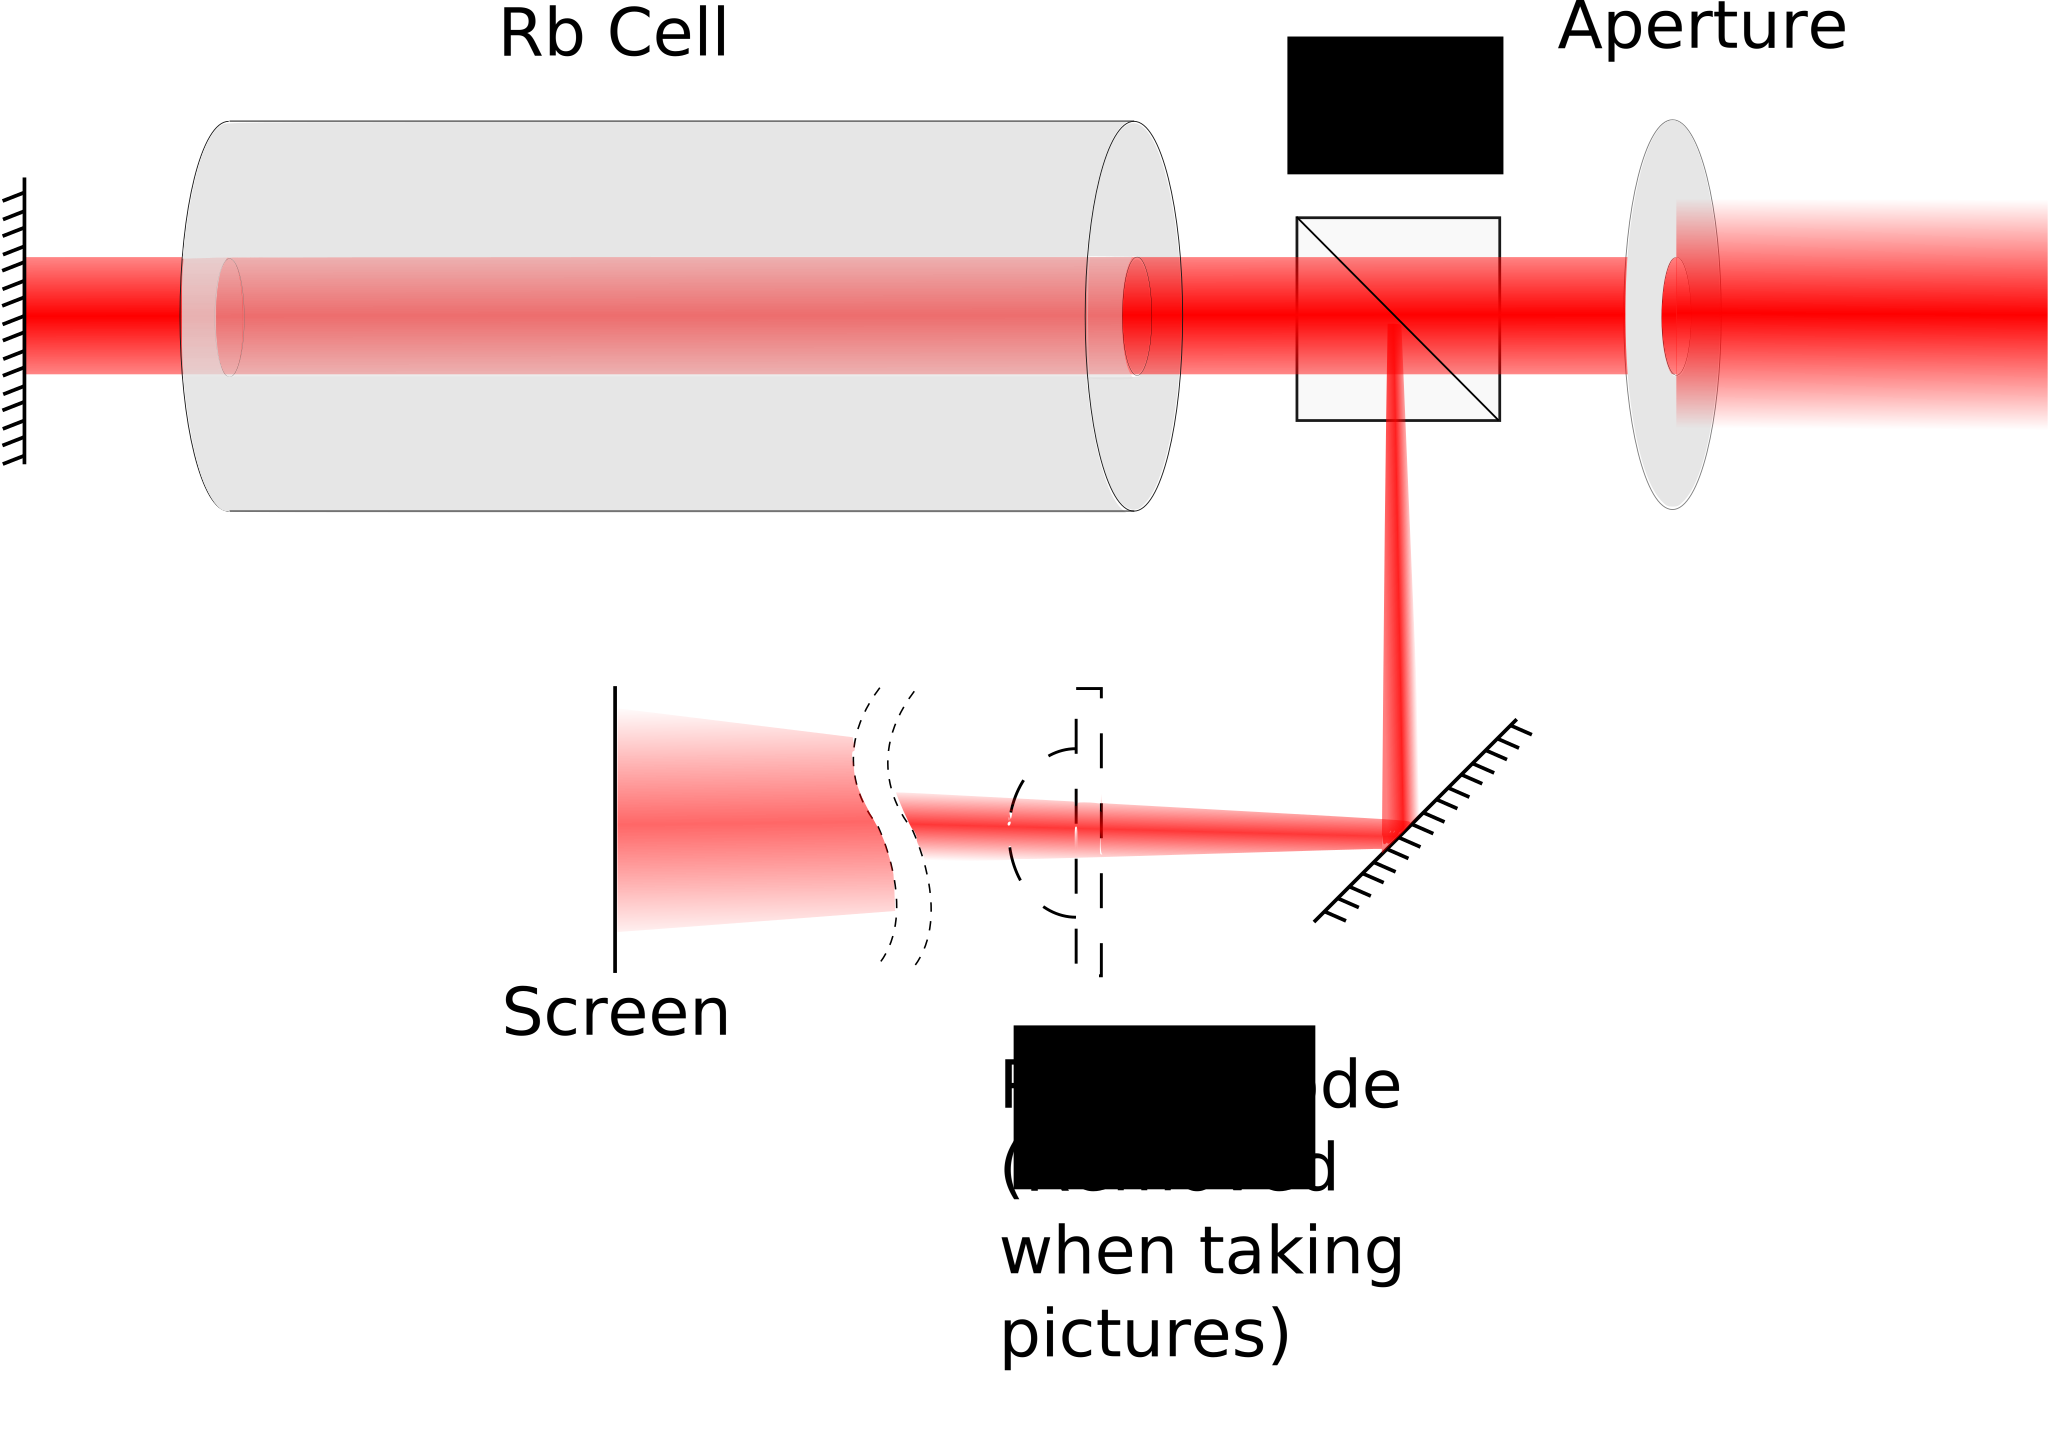
\includegraphics[width=9cm]{apparatus.png}
  \caption{Beam path setup of the experiment. The aperture is used to make the elliptical beam coming out of the diode laser more circular. The polarization beam splitter (PBS) is used to split the weak generated light with an orthogonal polarization from the main beam. A photo diode can be put in the beam path to measure the power helping to find the resonance frequency.}
  \label{apparatus}
\end{figure}

Figure \ref{apparatus} shows the setup of the main beam path in this experiment. The polarization beam splitter (PBS) is used both to clean up the polarization going into the cell and to select the generated light which has a polarization orthogonal to the incident beam. A photo diode is used to measure the power of the generated light to help searching for the signal. An aperture is also place in the beam to provide more symmetry to the system by making the elliptical beam coming out of the diode laser more symmetric. Since the generated pattern only has a small angle with the original beam, we put a screen far away ($2-3m$) from the cell to get a better resolution and record it using a camera.

\subsection{Heater design.}
The non-linear effect can only appear above certain atom density threshold. In order to reach the threshold, we need to increase the vapor pressure of the rubidium by increasing the temperature. We heat the cell by wrapping heating tape on the cell. The tape is only wrapped on the end of the cell so the window temperature can be kept higher than the middle of the cell to prevent condensation of atom on the optical window. In order to lower the magnetic field generated from the heating tape, we wrap it around the cell in both directions.

\section{Measurements and results}
\subsection{Generated light in the orthogonal polarization.}
\begin{figure}
  \includegraphics[width=9cm]{../data/5-16_csv/intensities.png}
  \caption{Power of light split from the cube that has a polarization orthogonal and parallel to the polarization of the incident beam when scanning the frequency of the laser.}
  \label{intensities}
\end{figure}

Figure \ref{intensities} shows the power of light split from the cube with either a polarization orthogonal or parallel to that of the incident beam during frequency scan of the diode laser measured by putting in the photo diode as shown in figure \ref{apparatus}. The light that has a polarization parallel to the incident beam is just a saturated absorption spectroscopy signal that is leaking through the cube since the cube is not ideal. The light with a orthogonal polarization is a combination of the leaking-through spectroscopy signal and the generated light signal. The difference in shape between the two signals clearly shows that we have generated light in this process.

\subsection{Interference rings for red detuned light.}
\begin{figure}
  \includegraphics[width=7cm]{rings.png}
  \caption{Interference rings taken from the screen for a large red detuning ($\approx 200MHz$). Multiple rings correspond to different hyperfine splittings can be seen.}
  \label{rings}
\end{figure}
\begin{figure}
  \includegraphics[width=9cm]{../data/5-16/ring-fit.png}
  \caption{Fitting of rings diameter with scan voltage.}
  \label{ring_fit}
\end{figure}

Figure \ref{rings} shows the pattern we have measured on a screen $3.1m$ away from the cell for a large red detuning ($\approx 400MHz$). Multiple interference rings can be observed (although only the smallest one is bright enough to be measured). These multiple rings are due to the fact that the Rubidium atoms we are using has more than one hyperfine levels and each of the hyperfine splitting line can create a interference ring as long as the diameter is small enough so it is not absorbed by the atoms that are not pumped by the laser. By fitting the diameters to the scan voltage, the frequency of the line is $386(37)THz$ which is within one $\sigma$ from $384THz$, the expected frequency for $780nm$ laser. We also determined from the fit the resonance point of the line we are measuring appears at scan voltage of $16.15(10)V$ and this is used in the experiment to find out the resonance point of the photo series we took.

\subsection{Flower like patterns}
\begin{figure}
  \includegraphics[width=7cm]{cone.png}
  \caption{Ring pattern generated at a smaller detuning and lower temperature.}
  \label{cone}
\end{figure}
For a higher laser power, smaller detuning ($<200MHz$) and lower temperature ($70.0^{\circ}C$) (therefore lower atom density), we saw a symmetric ring pattern as shown in figure \ref{cone}. The ring has a diameter of $3\pm1mrad$ which is close to what we expect from previous results $5mrad$ \cite{rb_switch}.

\begin{figure}
  \subfigure[$4$ spots]{
    \includegraphics[width=5cm]{flower1.png}
    \label{flower1}
  }
  \subfigure[$2$ spots]{
    \includegraphics[width=5cm]{flower2.png}
    \label{flower2}
  }
  \subfigure[$6$ spots]{
    \includegraphics[width=5cm]{flower3.png}
    \label{flower3}
  }
  \caption{Flower like patterns appears at a higher temperature ($\approx100^\circ C$) and smaller detuning ($<200MHz$). Figure \ref{flower1} \ref{flower2} \ref{flower3}, shows different mode of the generated light with $4$, $2$ and $6$ spots.}
  \label{patterns}
\end{figure}

By increasing the temperature to $\approx100^\circ C$ and therefore increase the atom density and non linearity, we can see the ring we saw at a lower temperature is broken into several different spots.

Figure \ref{patterns} shows the different mode of the generated light we can see in the experiment. Since our experiment do not have a really stable and isolated setup, the generated pattern are constantly rotating and changing between different mode. This shows that the patterns appears because of the small symmetry breaking in the system and is also sensitive to small ambient light, which is an important feature for making a all-optics switch.

\section{Conclusion}
In this experiment, we explored the non-linear effect in a rubidium vapor cell for close resonance beam. In particular, we studied the pattern in the generated light with an orthogonal polarization with the original beam. We have successfully seen interference rings as well as flower like patterns in the light and the results agree with what we expect very well.

Because of the limitation of equipment, we do not have a perfect stable setup to observe a precise relation between the flower like pattern generated and the detuning of the light. The input mode of the laser is also not a single Gaussian mode and this also affect the result. To get a better and more reliable result, we might need to use a more stable setup and also clean up the mode of the laser using either pin hole or fiber.

\bibliography{report}
\end{document}
